In this section, we evaluate the proposed algorithms on two  datasets and compare the results to two well known graph isomorphism detection algorithms. The first dataset is a set of synthetic data consisting of several graph databases featuring one of several fixed edge densities, label counts and total database graph count. We call his the synthetic dataset. The second dataset is  a set of graphs modeling active ingredients in antiviral drugs for the treatment of AIDS. We call this the AIDS dataset. 

We perform tests to evaluate the effect of several dataset parameters on the processing time.

We perform two sets of tests; In the first set, we evaluate 
our algorithms on the retrieval of induced subgraph to query and In the second set, we evaluate retrieval of non induced sugraph to query.  
To test the efficacy of our algorithm with regard to induced subgraph query, we evaluate the proposed algorithm in comparison with Messmer's Network Algorithm and a sequential SCAN using the state-of-the-art subgraph isomorphism detection algorithm VF2\cite{cordella2001_vf2}.
We also evaluate our algorithm with regard to non-induced subgraph query, where we compare proposed algorithm with the sequential scan only.
All the algorithms were implemented using the C++ programming language and run on a Intel Core i-3 CPU 3.09 GHZ, 16 Gbyte memory, Personal Computer running Windows 7 Professional Operating system.

\subsection{Graph Datasets}
We evaluate our algorithms by processing the retrieval of descriptors from the compounds dataset.
We use AIDS Antiviral Screen dataset to provide a real graph dataset.
This dataset contains around 43,000 chemical compounds and is available publicly from NCI
\footnote{National Cancer Institute http://dtp.nci.nih.gov/}.
We denote this dataset as ``AIDS'' in our experiment.
The graphs of AIDS have an average number of 25 vertices and 27 edges, a maximum of 438 vertices and 441 edges,
63 distinct vertex labels and 3 distinct edge labels.

In order to evaluate our algorithms over a larger database to test scalability, we use synthetic large dataset. 
The graph generator is configured to emit only connected graphs thathave an edge probability of 50 percent. 
Except where explicitly stated, 10 distinct vertex labels and 10 distinct.

\begin{figure}[h]
\centering
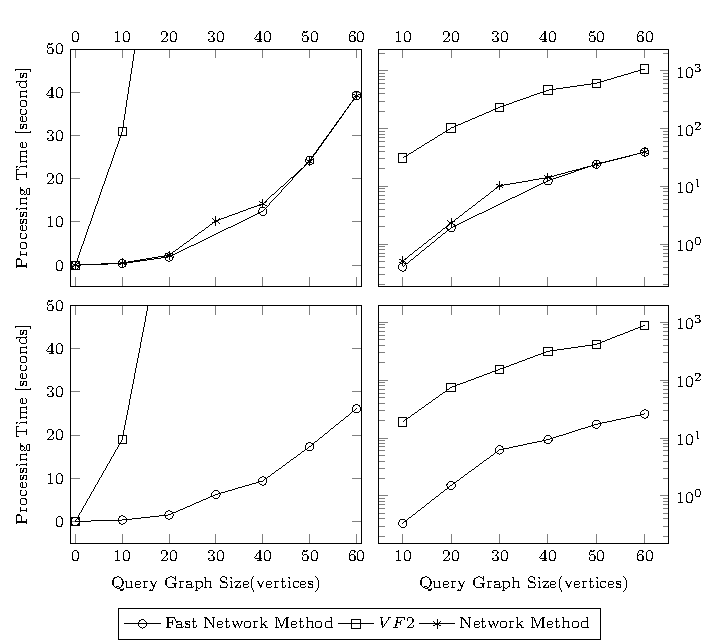
\includegraphics[width=1.0\textwidth]{images/realdataplot.pdf}
\caption{\textbf{Results of the Experiments on the Real World Graph Data Set} 


\textbf{ Top left:}Linear-linear plot of  induced subgraph query processing time for increasing size of query graph.The smallest query graph contains 10 vertices while the largest query graph contains 60 vertices. The \textit{Fast Network Method} and the textit{Network Method} show almost identical processing times. The \textit{VF2} method is noticably slower. 


\textbf{Top Right:} Linear-log plot of the induce subgraph graph query processing time with query graph size. The \textit{Fast Network Method} and the textit{Network Method} are almost indistinguishable and show an order of magnitude advantage over the state-of-the-art \textit{VF2} Method 

\textbf{ Bottom left:}Linear-linear plot of  query processing time for increasing size of graph query. The smallest query graph contains 10 vertices while the largest query graph contains 60 vertices. The \textit{Fast Network Method} is faster than \textit{VF2} for subgraphs as well. The \textit{VF2} method takes more than 50s to process query graphs large than 10 vertices. 

\textbf{Bottom Right:} Linear-log plot of the graph query processing time with query graph size. Both the \textit{Fast Network Method} and the textit{Network Method} are almost indistinguishable and show more than an order of magnitude advantage over the \textit{VF2} Method.}

\label{fig:fig81}
\end{figure}

\subsection{Chemical Descriptor Search}
In chemistry, substructures of compounds that imply a chemical, physical property of the compound are called as descriptor.
Fast retrievals of descriptors from compounds aids research of compounds.
We evaluate our algorihm by processing the retrievals of descriptors.
We builded a model graph database $D$ by extracting graph database $W$ composed of 10,000 compounds whose size are less than 40 from AIDS and applying frequent graph mining to $W$.
We set minimum support as 5 percent.
$D$ is composed of 18930 distictive frequent subgraphs.

We vary average size of query graphs and evaluate query processing time.
For each plot, 100 query graphs are extracted from $W$.
Query processing time is time to process the all query graphs and the time to construct the DAG is excluded. In the results we compare the processing time of two methods with our proposed \textit{Fast Network Algorithm}. These methods are: 

The \textit{Network algorithm}, in which the use of $DAG$ data structure to store the graphs was pioneered. This method however was only implemented for induced subgraph queries, so we are only able to perform comparisons for half of the experiments. 

The state-of-the-art one-on-one graph query algorithm \textit{VF2}. This algorithm  tests a graph for subgraph isomorphism or induced subgraph isomorphism to another single graph only. This is repeated sequentially for a large graph database. The solution is a binary true or false answer. It cannot be used to find all isomorphisms to a graph in a database as one is not able to differentiate multiple isomorphisms from a binary response.

We now analyse the results.

The  top left of Fig.\ref{fig:fig81} shows a Linear-linear plot of induced subgraph query processing time for increasing size of query graph. In this experiment, the smallest query graph contains 10 vertices while the largest query graph contains 60 vertices. For this real world graph database the \textit{Fast Network Method} and the textit{Network Method} show almost identical processing times. In this evaluation \textit{VF2} method is the slowest, taking more than 50 seconds to process query graphs containing more than 10 vertices. The fact that the \textit{Fast Network Method} is not substantially better than the \textit{network Method} implies that we do not have many fragmented graphs during decomposition, hence there is no advantage in ensuring that all decomposed graphs are connected.  

Top Right of Fig.\ref{fig:fig81} shows a Linear-log plot of the induce subgraph graph query processing time with query graph size. We observe that both the \textit{Fast Network Method} and the textit{Network Method}, while almost indistinguishable, show an order of magnitude advantage in processing time over the state-of-the-art \textit{VF2} Method. 

Bottom left of Fig.\ref{fig:fig81} shows a Linear-linear plot of  query processing time with increasing  time in the  graph query. The experiment was performed using query graphs containing 10 vertices to 60 vertices. Here \textit{Fast Network Method} is faster than \textit{VF2} for subgraphs too. We also observe that the \textit{VF2} method takes more than 50s to process query graphs large than 10 vertices. 

Bottom Right of Fig.\ref{fig:fig81} shows a Linear-log plot of the graph query processing time with increasing query graph size. We observe that both the \textit{Fast Network Method} and the \textit{Network Method} while almost indistinguishable, show more than an order of magnitude advantage in processing time over the state-of-the-art \textit{VF2} Method.}

It is because that their are originally few decompositions that creates disconnected graphs and also few redundant subgraph isomorphism detections in DAG.
So in this experiment, our improvements did not work.

Fig.\ref{fig:fig4} shows the processing time for subgraph isomorphism query.
Fig.\ref{fig:fig4} indicates the subgraph isomorphism query is faster than SCAN same as Messmer et al's algorithm.

\begin{figure}[h]
\centering
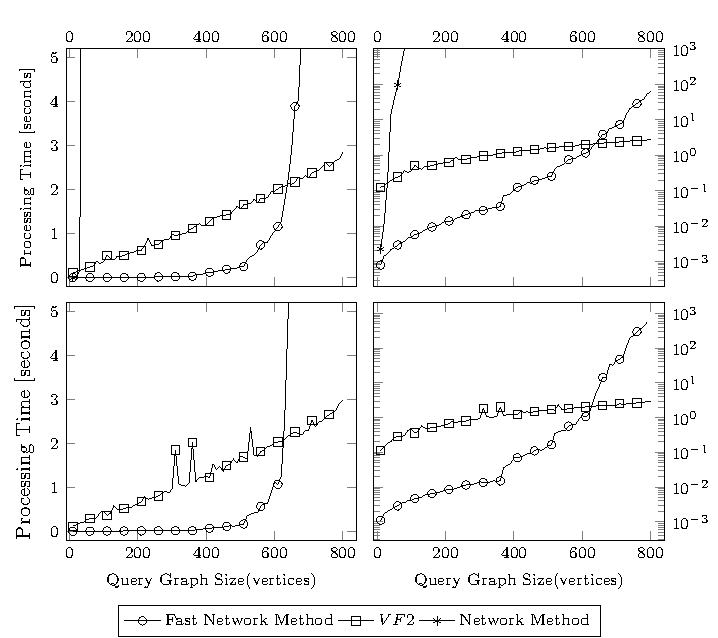
\includegraphics[width=1.0\textwidth]{images/syndataplot.pdf}
\caption{\textbf{Results of the Experiments on the Synthetic Graph Data Set} 

\textbf{ Top left:}Linear-linear plot of induced subgraph query processing time against query graph vertex count. The query graph size ranges from 10 vertices to 800 vertices. The \textit{Fast Network Method} and the \textit{Network Method} show the fastest processing time for induced subgraph queries of up to 600 vertices. For larger query graphs, the \textit{VF2} method is faster. The \textit{Network Method} takes more than 5sec for any induced subgraph query graph greater than 10 vertices. The \textit{VF2} method shows an almost linear time dependency of query graph vertex count, an advantage for induced subgraph queries larger than 600 vertices. 

\textbf{Top Right:} Linear-log plot of the induce subgraph graph query processing time with query graph size. We observe that for induced subgraph query size less than 400 Vertices, there is an order of magnitude or better advantage to the \textit{Fast Network Method}. Beyond query graphs of about 600 vertices the \textit{VF2} method is clearly superior. We observe that the \textit{Network Method} is slowest, taking about 15min for an induced subgraph query of just 80 vertices.

\textbf{ Bottom left:}Linear-linear plot of  query processing time for increasing size of graph query.The smallest query graph contains 10 vertices while the largest query graph contains 800 vertices. The \textit{Fast Network Method} processes query graphs faster than \textit{VF2} for subgraphs not larger than 600 vertices. Here too, \textit{VF2} method shows an almost linear processing time  dependency with query graph size.  

\textbf{Bottom Right:} Linear-log plot of the induce subgraph graph query processing time with query graph size. For subgraph query size less than about 400 Vertices, there is an order of magnitude or better advantage to the \textit{Fast Network Method}. For synthetic graphs of less that 50 vertices, the advantage is about two orders of magnitude. Beyond query graphs of about 600 vertices the \textit{VF2} method is superior.
}
\label{fig:fig91}
\end{figure}
%

\subsection{Synthetic Data Search}
In chemical descriptor search, we can not show improvements of proposed algorithm in term of processing time.
In order to demonstrate improvements of proposed algorithm, we process subgraph isomorphism query on synthetic data.

We vary average size of query graphs and evaluate query processing time.
Model graph dataset is composed of 20,000 graphs whose average number of size are 10.
100 query graphs are generated for each plot.



Fig.\ref{fig:fig5} shows the processing time for induced subgraph isomorphism query.
Fig.\ref{fig:fig5} indicates that proposed algorithm is faster than Messmer et al.'s algorithm.
The processing time of proposed algorithm is stable against the variation of the size of query graphs.
On the contrary, the processing time of Messmer et al.'s algorithms is skyrockets when the size of query graphs becomes large.

%\begin{figure}[h]
%\centering
%\epsfig{file=images/Typ_Syn_Siz_Pro.eps, height=2in, width=3in}
%\caption{Processing Time for typical Subgraph Isomorphism Query}
%\label{fig:fig6}
%\end{figure}

%


%\begin{figure}[h]
%\centering
%\epsfig{file=images/Ind_Syn_DAG_Con.eps, height=2in, width=3in}
%\caption{DAG Construction Time for Induced Subgraph Isomorphism Query}
%\label{fig:fig7}
%\end{figure}

We vary size of model graph database and evaluate the construction time of DAG.
Fig.\ref{fig:fig7} shows the construction time of DAG for induced subgraph isomorphism query.
The construction Time of DAG of proposed algorithm is almost same as the one of Messmer et al.'s algorithm.

%% \Subsection{Appendix}


%% \begin{algorithm}
%% \caption{New Network Algorithm, NNA($D , q$)}
%% \label{alg:alg05}
%% \begin{algorithmic}
%% \STATE Input: Model graphs in DAG, $D(G)= \{$($g_1 ,s_1 ,P_1 ,\{c^{'}_1 ,c^{''}_1 \},E$)$,\ldots,$($g_n,s_n,P_n,\{c_n^{'},c_n^{''}\},E_n$)$ \}$, Query $q$
%% \STATE and the set of all subgraphs in DAG, $G_{all} = \cup_{i=1}^n \{g_1 ,c_1^{'},c_1^{''},g_2 ,c_2^{'},c_2^{''}\ldots \}$ 
%% \STATE Output: $Z$, the set of all subgraph isomorphisms in Model graphs in $D$ to query $q$ 
%% \end{algorithmic}
%% \begin{algorithmic}[1]
%% \STATE $F \leftarrow \emptyset$
%% \STATE $Z \leftarrow \emptyset$
%% %%\FOR{ each $(g,s,P,\{c^{'},c^{''}\}) \in  D$}
%% \FOR{ each subgraph in $G_{all}$}
%%   \STATE  $s \leftarrow unsolved$
%% \ENDFOR
%% \FOR{ each $(g,s,P,\{c^{'},c^{''}\}) \in D$}
%%    \STATE $F \leftarrow $SubgraphQuery($g,s,P,\{c^{'},c^{''}\},q$)
%%    \IF{$F\neq \emptyset$}
%%       \STATE $Z \leftarrow Z \cup \{F\}$
%%    \ENDIF
%% \ENDFOR
%% \RETURN $Z$
%% \end{algorithmic}
%% \end{algorithm}


% LocalWords:  kna
